%导言区
\documentclass{report}
\usepackage{graphicx}
\usepackage{subfigure}
\usepackage{caption}
\usepackage{wrapfig}
\graphicspath{{latex report/}}


%正文区
\begin{document}
\begin{figure}
\section{Bonus}
~\\
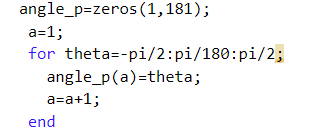
\includegraphics[scale=1]{创建角度数组}
\\Create an array of angles, traversing -pi/2 to PI /2, that is to create the abscissa of the plot.
\end{figure}
~\\
\begin{figure}
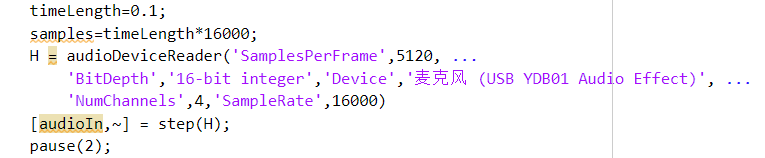
\includegraphics[scale=1]{设置初始值}
\\Set the sampling time to 0.1 seconds.
\\The default sampling rate was 44,100, and calculate the number of sampling points.
\\The recording data length per treatment was set with the audioDeviceReader function to be 5,120, the number of microphone channels was 4 channels, and the sampling frequency was 16,000HZ
This function serves to constantly record and process the data in real time.
\end{figure}
~\\
\begin{figure}
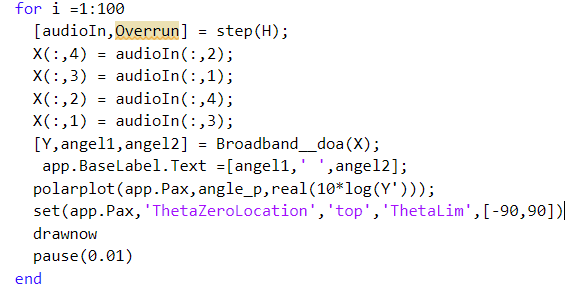
\includegraphics[scale=1]{录音}
\\We found that the order of the microphone was not the same correspondence of the array obtained from the recording, so the order was modified.
\\The Broadband doa function is called to derive the P value and  the directions of two sound sources.
\\Create an app.Firstly, set the two angles that can be displayed on the app.
\\Secondly, draw the image of the polar coordinates and set the abscissa and ordinate.
\\Thirdly, take the image of the polar coordinates in the upper half and set the angle to range from-90°to 90 °.

\end{figure}
~\\
\begin{figure}
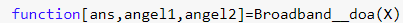
\includegraphics[scale=1]{broadband doa}
\\This is the Broadband doa mentioned above
\end{figure}
~\\
\begin{figure}
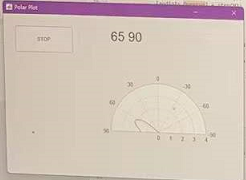
\includegraphics[scale=1]{app}
\\This is the displaying interface of our app.
\end{figure}

\begin{figure}
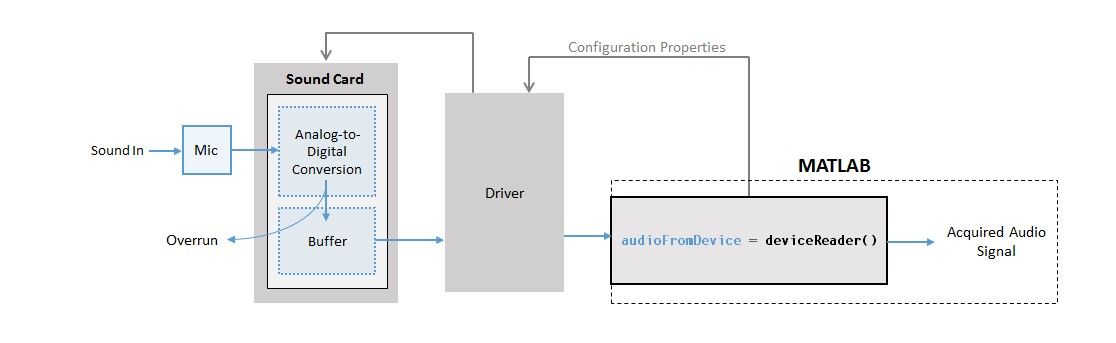
\includegraphics[scale=0.5]{audiodevicereader}
\\The principle of AudioDeviceReader: after the sound enters, after the ADC processing, cache first, excess and then overflow.It acts as recording, storing recording and processing recording.
\end{figure}

\begin{figure}
Error analysis

1.Planar wave means that the distance between the microphone is far less than the sound source to the microphone, but we measure it as equivalent to a spherical wave, and we treat it as a plane wave, which causes error.

2.The direction of the sound source is not in the same reference plane as the microphone,so the source has an elevation relative to the microphone, but the microphone default source is within the reference plane.
\end{figure}

\end{document}